% !TEX root = ../../presentation.tex
% Meta: Erster Teil

\textframe{\texttt{.meta}}

% Stand der Welt vor einem Jahr, wie haben wir die Welt, im kleinen, seit dem veraendert
% !TEX root = ../../presentation.tex
% Meta: Intro

\textframe{\texttt{.meta}}

\begin{slide}{Vorgeschichte}
  \scalebox{1.5}{
    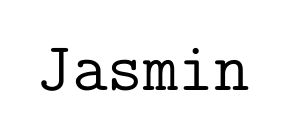
\begin{tikzpicture}
      \node at (0, 0) {\Huge\texttt{Jasmin}};

      \onslide<2->{
        \node at (-1.26, 0.37) [rotate=45] {\color{red}\tiny\PHhorn};
      }

      \onslide<2->{
        \node at (-0.84, 0.37) [rotate=-45] {\color{red}\tiny\PHhorn};
      }
    \end{tikzpicture}
  }
\end{slide}


% Jasmin blablabla, wir haben dann die Aufgabe bekommen, mit C++ und Qt einen neuen Simulator zu entwickeln, dessen Ziel es war, viele der Schwachstellen von Jasmin durch ein besseres Design und einer besseren Implementierung zu umgehen. Apropros Ziele: Jedes grosse Projekt braucht natuerlich drei Dinge: eine Vision, einen Plan und die Exekution. Unsere Vision war ...
% !TEX root = ../team-report.tex
% ERA-Großpraktikum: Team Bericht -- Organisatorisches (Vision)

\subsubsection{Die Vision}
\label{team:orga-plan-vision}
\vspace{-0.2cm}

In den ersten sechs bis acht Wochen des Großpraktikumszeitraums beschäftigte
sich die Gruppe mit der Ausarbeitung eines groben Grundrisses für die
Architektur des Simulators, mit der Gewöhnung an die notwendigen Technologien
für die Implementierung sowie mit der Definition einer Vision und eines
Zeitplanes. Die Vision war primär von zwei Quellen beeinflusst. Zum einen waren
dies unsere eigenen Erfahrungen als Studierende in der Vorlesung
\emph{Einführung in die Rechnerarchitektur} (ERA). Da jeder von uns gerade erst
in derselben Situation wie unsere zukünftigen Kunden gesessen hatte, konnten wir
natürlich leicht spezifizieren, was uns und unseren Kommilitonen beim Erlernen
der maschinennahen Programmierung und Assemblersprachen geholfen hätte. Zum
anderen hatten wir durch den bereits existierenden und von uns in ERA genutzten
Simulator einen Referenzpunkt für die Entwicklung von \erasim{}. Wir konnten
analysieren, welche Aspekte von Jasmin uns geholfen hatten, konnten aber
insbesondere auch jene Features nennen, welche uns an Jasmin nicht gefielen und
deren Verbesserung als Ziel für \erasim{} festlegen.

Die Überlegungen dieser ersten Phase verfestigten sich schließlich in den
folgenden langfristigen Zielen:
\begin{senumerate}{-0.45cm}
  \item Die Funktionen von \erasim{} sollten eine Übermenge jener von Jasmin
  sein. Das bedeutet, dass sämtliche Aufgaben aus früheren Zentralübungen,
  Klausuren und Tutorübungen (soweit in RISC-V übersetzbar) in unserem Simulator ausführbar sein sollten.
  \item Der Simulator soll zwar primär für die Lehre gedacht, jedoch nicht durch
  diese beschränkt sein. Auch weitere Einsatzgebiete, wie die Forschung,
  sollten, zumindest durch Erweiterungen der Grundversion, offen bleiben. Eine
  Grundanforderung hierfür war es, echte RISC-V Programme ausführen zu können.
  \item Als Voraussetzung für (2) sollte der Simulator nicht \emph{zeilen}-,
  sondern \emph{address}basiert sein. Das bedeutet, dass Marken Adressen im
  Speicher und nicht Zeilen im Text referenzieren sollten. Hierfür müssten
  Instruktionen auch in den Speicher assembliert werden.
  \item Als wohl wichtigste Eigenschaft sollte \erasim{}, im Vergleich zu
  Jasmin, nicht nur für einen bestimmten Befehlssatz wie x86 oder ARM
  implementiert sein, sondern für beliebige Architekturen erweiterbar bleiben.
  \vspace{-0.4cm}
\end{senumerate}


% Wir haben also einen RISC-V Simulator als erste Implementierung entwickelt.
% RISC-V ist, wie Sie alle wissen, eine modulare Architektur, was auch ihre
% Staerke ist. Projekt einschraenken --- nein eingrenzen.
% Durch unser modulares Design erfordert die Erweiterng des Simulators kein
% neues Design oder Neustrukturierung, sondern ist vollkommen eine Funktion von
% Zeit. Gegeben mehr Zeit, koennen ohne Einschraenkungen neue Komponenten dem
% Simulator hinzugefuegt werden.
\chapter{RISC-V}

In diesem Teil der Spezifikation wollen wir die grundlegenden Eigenschaften und
Eigenheiten der RISC-V (``RISC-Five'') instruction-set-architecture (ISA)
erläutern. Wir beginnen mit einer kurzen Einführung in die wichtigsten
Bestandteile des Befehlssatzes. Anschließend fokussieren wir uns auf eine
Diskussion der Unterschiede zwischen RISC-V und x86. Wir nehmen an, dass der
Leser vor allem mit x86 Erfahrung hat und wollen den Umstieg durch diese Sektion
erleichtern.

\section{Die RISC-V ISA}

RISC-V ist ein neuer quelloffener Befehlssatz, der
ursprünglich zu Lern- und Forschungszielen entwickelt wurde.

Es gibt zwei Versionen mit 32-Bit- und 64-Bit-Architektur. Wir werden
vorerst ausschließlich erstere Variante betrachten.

Die Architektur ist in Module auf geteilt, die nach zu einer Konfiguration nach Belieben hinzugefügt werden können.
Lediglich das Basismodul für Ganzzahloperationen ``I'' (Basic Integer Module) muss dabei in allen Implementierungen vorhanden sein.
Es enthält Rechen-, Lade-, Speicher- und Kontrollflussbefehle auf ganzzahlige Werte und kann durch folgende
Standardmodule erweitert werden:

\begin{itemize}
\item ``M'' Multiplikation und Division für ganze Zahlen
\item ``A'' atomare Operationen für prozessorübergreifende Synchronisation
\item ``F'' und ``D'' für Gleitkommazahlen einfacher und doppelter Genauigkeit (floats und doubles)
\end{itemize}

Die Instruktionen des Standardbefehlssatzes sind 32 Bit lang und auf
32-Bit-Grenzen ausgerichtet. Jedoch unterstützt RISC-V auch Befehle variabler Länge, die
aus einer beliebigen Anzahl von 16-Bit-Blöcken bestehen können.

Standardmäßig wird Little-Endian als Speicherformat verwendet.

Die RISV-V ISA hat 31 Allzweckregister (\lstinline[style=risc-v_Assembler]!x1! bis \lstinline[style=risc-v_Assembler]!x31!). Zusätzlich existiert das Register \lstinline[style=risc-v_Assembler]!x0!, der mit einer konstanten \lstinline[style=risc-v_Assembler]!0! verdrahtet ist sowie der Befehlszähler (ab sofort abgekürzt mit \lstinline[style=risc-v_Assembler]!pc!). All diese Register sind 32 Bit breit.

\subsection{Binärdarstellung}

Jeder Befehl im RISC-V Simulator wird zur Kompilierzeit in seine
Binärdarstellung umgewandelt und in den Speicher reingeschrieben. Unser Model
ist also addressbasiert. Und das ermöglicht unserem Programm evtl. Obj-Dateien
einzulesen und sie zu interpretieren.

\subsection{Grundlegende Ganzzahl-Befehle (Integer Basic Module)}

Rechenbefehle auf ganzen Zahlen verursachen keine arithmetischen Ausnahmen.

\subsubsection{Register-Unmittelbar}

\begin{lstlisting}[style=risc-v_Assembler]
ADDI rd, rs1, 0  ; (add immediate) addiert die Konstante und den Wert von r1, das ganze wird dann nach rd gespeichert
SLTI rd, rs1, 0  ; (set less than immediate) setzt den Wert von rd=1, falls rs1 < 0, sonst rd=0
SLTIU rd, rs1, 1 ; (set less than immediate unsigned) wie SLTI, nur vorzeichenloser Vergleich
\end{lstlisting}

\lstinline[style=risc-v_Assembler]!ANDI!, \lstinline[style=risc-v_Assembler]!ORI!, \lstinline[style=risc-v_Assembler]!XORI! sind logische Operationen, die dem bitweisen Und, Oder bzw. Exklusiv-Oder entsprechen (Register-Register-Äquivalent: \lstinline[style=risc-v_Assembler]!AND!, \lstinline[style=risc-v_Assembler]!OR! bzw. \lstinline[style=risc-v_Assembler]!XOR!). Ihr
Befehlsformat entspricht dem obigen. \textbf{Was meintet ihr mit "entsprechen AND, OR, und XOR?"}

Zudem existieren logische und arithmetische Shifts (\lstinline[style=risc-v_Assembler]!SLLI!, \lstinline[style=risc-v_Assembler]!SRLI!, \lstinline[style=risc-v_Assembler]!SLAI!, \lstinline[style=risc-v_Assembler]!SRAI!). Die Anzahl
der geshifteten Bits ist gleich der Zahl, die aus den ersten fünf Bits der angegebenen Konstante entsteht.

In den nächsten beiden Befehlen ist die unmittelbar angegebene Konstante 20 Bit lang, anstatt 12 Bit.

\begin{lstlisting}[style=risc-v_Assembler]
LUI dest, immediate  ; (load upper immediate)
AUIPC dest, immediate  ; (add upper immediate to program counter)
\end{lstlisting}

\lstinline[style=risc-v_Assembler]!LUI! platziert die Konstante in die höheren 20 Bits des Zielregisters, die unteren 12 Bits werden genullt.

\lstinline[style=risc-v_Assembler]!AUIPC! addiert die Konstante mit den höheren 20 Bits des Befehlszählers und speichert das Ergebnis in das Zielregister.

\subsubsection{Register-Register}

\begin{lstlisting}[style=risc-v_Assembler]
ADD/SLT/SLTU dest, src1, src2
AND/OR/XOR   dest, src1, src2
SLL/SRL      dest, src1, src2
SLA/SRA      dest, src1, src2

SLTU rd, x0, rs2 ; (set less than unsigned) setzt rd zu 0, nur wenn rs2 = 0 (da x0 auf 0 fest verdrahtet ist)
\end{lstlisting}

\subsubsection{NOP-Instruktion}

\begin{lstlisting}[style=risc-v_Assembler]
ADDI x0, x0, 0
\end{lstlisting}

\subsubsection{Unbedingte Sprünge}

\begin{lstlisting}[style=risc-v_Assembler]
JAL rd, immediate  ; rd = (pc + 4), Konstante (immediate) ist 20 Bit lang, Bereich: +-1MiB
\end{lstlisting}

\lstinline[style=risc-v_Assembler]!JAL! (jump and link) speichert \lstinline[style=risc-v_Assembler]!pc + 4! (Befehlszähler um 4 vorgeschaltet) in das Register rd und setzt anschließend den Befehlszähler auf \lstinline[style=risc-v_Assembler]!pc+imm! (Befehlszähler + Konstante). Somit kann der Wert in rd als Rücksprungadresse dienen. Die Konvention ist, dass man diese normalerweise nach x1 speichert. Wenn aber nicht zurückgesprungen werden soll, so kann die Rücksprungadresse auch auf \lstinline[style=risc-v_Assembler]!x0! (die fest verdrahtete \lstinline[style=risc-v_Assembler]!0!) geschrieben werden und geht verloren.

\begin{lstlisting}[style=risc-v_Assembler]
JALR rd, rs1, immediate  ; rd = (pc + 4), die Konstante (immediate) 12 Bit lang
\end{lstlisting}

\lstinline[style=risc-v_Assembler]!JALR! setzt den Befehlszähler auf \lstinline[style=risc-v_Assembler]!rs1 + imm! (Quellregister 1 + Konstante). Zusammen mit dem Befehl \lstinline[style=risc-v_Assembler]!LUI! kann
man damit auf eine beliebige Adresse im Adressraum springen.

\subsubsection{Bedingte Verzweigungen}

Ein wichtiger Aspekt des RISC-V-Befehlssatzes ist, dass es weder Flags noch ein Statusregister gibt. Stattdessen
werden Verzweigungsbefehle verwendet:

\begin{lstlisting}[style=risc-v_Assembler]
BEQ/BNE src1, src2, offset ; (branch equal/not equal)
BLT[U]/BGE[U]  src1, src2, offset  ; (branch less/greater than)
\end{lstlisting}

Falls die Bedingung erfüllt ist, wird \lstinline[style=risc-v_Assembler]!offset! zu dem Befehlszähler addiert.

\subsubsection{Lade-/Speicher-Instruktionen}

\begin{lstlisting}[style=risc-v_Assembler]
LW/LH/LB rd, rs1, offset ; (load word/half/byte) kopiert 32/16/8 Bits vom Speicher von der Adresse (rs1+offset)
SW/SH/SB rd, rs1, offset ; (store word/half/byte) kopiert den Wert von rd in den Speicher
\end{lstlisting}

Neben \lstinline[style=risc-v_Assembler]!LH! und \lstinline[style=risc-v_Assembler]!LB! existieren auch \lstinline[style=risc-v_Assembler]!LHU! und \lstinline[style=risc-v_Assembler]!LBU! (analog \lstinline[style=risc-v_Assembler]!SHU!, \lstinline[style=risc-v_Assembler]!SBU!). Der Unterschied ist, dass der
kopierte 16-/8-Bit-Wert mit Nullen, hingegen bei \lstinline[style=risc-v_Assembler]!LH! und \lstinline[style=risc-v_Assembler]!LB! mit dem Vorzeichenbit auf 32 Bits aufgefüllt wird.

\subsection{Befehlsformate von RISC-V}

Wir stellen fest, dass es bei RISC-V nur wenige Befehlsformate gibt, in der Tat sind es genau vier:

\begin{itemize}
\item R-Typ --- Operation Ziel, Quelle 1, Quelle 2 (\lstinline[style=risc-v_Assembler]!opcode rd, rs1, rs2!)
\item I-Typ --- Operation Ziel, Quelle 1, Konstante (\lstinline[style=risc-v_Assembler]!opcode rd, rs1, immediate!)
\item S-Typ --- Operation Quelle 1, Quelle 2, Konstante (\lstinline[style=risc-v_Assembler]!opcode rs1, rs2, immediate!)
\item U-Typ --- Operation Ziel, Konstante (\lstinline[style=risc-v_Assembler]!opcode rd, immediate!)
\end{itemize}

Beim U-Typ ist die Konstante 20 Bit lang, sonst 12 Bit, da bereits zwei Register kodiert werden müssen.

\section{Unterschiede zwischen x86 und RISC-V}

In den folgenden Absätzen wollen wir die wichtigsten Unterschiede zwischen dem
x86 und RISC-V Befehlssatz erläutern. Wir möchten dadurch den übrigen
Teammitgliedern den Umstieg von x86 erleichtern sowie unsere eigenen
Beobachtungen festhalten.

\subsection{Load/Store Paradigma}

Ein grundlegender Unterschied zwischen RISC-V, als
reduced-instruction-set-comuting (RISC) ISA, und x86, als
complex-instruction-set-computing (CISC) Befehlssatz, ist die Beschränkung der
Zugriffsmöglichkeiten auf den Speicher. In x86 ist es erlaubt, bei so gut wie
jedem Befehl einen Speicherzugriff als Operand anzugeben, wobei aber die
Beschränkung auf nur einen solchen Zugriff gilt. So können wir beispielsweise
die folgenden wohl-geformten Befehle ausdrücken:

\begin{lstlisting}
  ; Schreibe den Wert an der Speicheradresse
  ; 0xDEADBEEF in das Register EAX
  mov eax, [0xDEADBEEF]
  ; Addiere den Wert im Register EAX auf den
  ; Wert an der Speicheadresse 0xDEADAFFE
  add [0xDEADAFFE], eax
\end{lstlisting}

In RISC-V wären diese Befehle nicht erlaubt, da es das LOAD/Store Paradigma
befolgt. Das bedeutet, dass nur zwei Instruktionen gibt, die auf den Speicher
zugreifen können: \code{LOAD} und \code{STORE} (in Pseudo-Code). Der erste
Befehl lädt ein einen Wert an einer Speicheradresse in ein Register. Im
Gegensatz dazu erlaubt \code{STORE}, einen Wert aus einem Register an eine
Speicheradresse zu legen.

Im RISC-V gibt es mehrere Varianten dieser beiden Befehlsklassen, für
verschieden breite Speicherzugriffe. Für LOAD, wären das:

\begin{itemize}
  \item \code{LW dest, base, immediate}: Lädt ein Wort (32-Bit für RV32I) an der
    Speicheradresse, die sich aus den oberen 20 Bit von \code{base} und der
    11-Bit Konstante \code{immediate} zusammensetzt.
  \item \code{LH[U] dest, base, immediate}: Lädt ein Halbwort
    (engl. \emph{halfword}; 16-Bit für RV32I) an der Speicheradresse, die sich
    aus den oberen 20 Bit von \code{base} und der 11-Bit Konstante
    \code{immediate} zusammensetzt. Für \code{LH} wird der geladene 16-Bit Wert
    sign-extended\footnote{Das bedeutet, dass negative Werte mit gesetztem MSB
      mit weiteren Einsen nach links aufgefüllt werden. Positive Werte, dessen
      Sign-Bit gelöscht ist, werden mit weiteren Nullen gepaddet.}, bevor er im
    Zielregister abgelegt wird. Bei \code{LHU}\footnote{Es gibt kein LWU, weil
      ein Wort schon die vollen 32-Bit belegt und man sich somit nicht um
      Erweiterung auf größere Datentypen kümmern muss.} (\emph{load halfword
      unsigned}) wird der Wert hingegen nur mit Nullen aufgefüllt.
  \item \code{LB[U] dest, base, immediate} Lädt wie \code{LH[U]} einen Wert von
    der gegebenen Speicheradresse in das Zielregister. Hierbei wird jedoch ein
    enziger \textbf{B}yte, also 8-Bit, geladen. Die übrigen 24 Bit werden wieder
    aufgefüllt, entweder mit dem Sign-Bit (\code{LB}) oder mit Nullen
    (\code{LBU}).
\end{itemize}

Wie kann man mit diesen Befehlen nun den gesamten 32-Bit Adressraum ansprechen?
Zuerst würde man dafür mit \code{LUI} (\emph{load upper immediate}) einen 20-Bit
Wert in ein Register legen und dieses Register dann als Basisregister
verwenden. Auf diese 20-Bit kann man dann eine beliebige 12-Bit Konstante
aufaddieren:

\begin{lstlisting}
  ; Wir wollen die Addresse 0xDEADBEEF nach Register x1 laden
  ; Zuerst geben wir die oberen 20 Bit in ein Register
  lui x2, 0xDEADB
  ; Dann benutzen wir x1 als Basis und addieren die unteren 12 Bit
  lw x1, x2, 0xEEF
\end{lstlisting}

Nun für Store:

\begin{itemize}
  \item \code{SW source, base, immediate}: Speichert den 32-Bit Wert in \code{source}
    an die Addresse \code{base + immediate}. Die Konstante \code{immediate} ist
    hierbei wieder 11-Bit.
  \item \code{SH} Speichert die unteren 16-Bit aus \code{source} an die Addresse
    \code{base + immediate}. Die Konstante \code{immediate} ist hierbei wieder
    11-Bit.
  \item \code{SB} Speichert die unteren 8-Bit aus \code{source} an die Addresse
    \code{base + immediate}. Die Konstante \code{immediate} ist hierbei wieder
    11-Bit.
\end{itemize}

Theoretisch erlauben die obigen Befehle auch \emph{unausgerichtete}
Zugriffe. Die RISC-V Architektur erlaubt solche Zugriffe, wobei die
Spezifikation jedoch anmerkt, dass sie für optimale Performance vermieden werden
sollten.

\subsection{Reduzierter Befehlssatz}



\subsection{Fehlende Flags}

\subsection{Instruktionsformate}

\subsection{Calling Conventions}

\subsection{Multiplikation und Division}



% Mit diesen Komponenten kann man jetzt also ein
% Rezept fuer einen Simulator entwickeln.
% !TEX root = ../../presentation.tex
% Meta: Module

\begin{slide}{Module}
  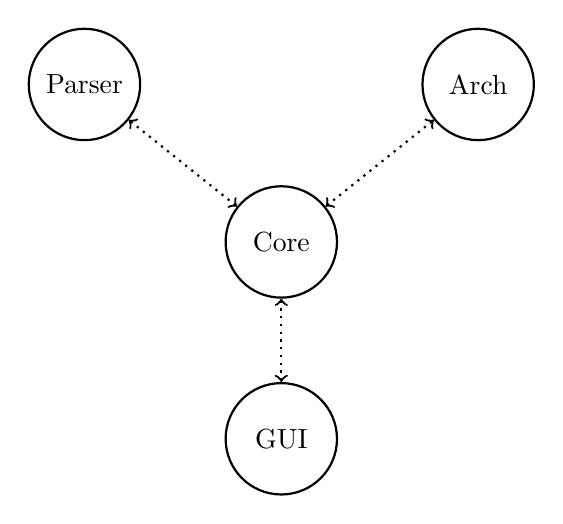
\begin{tikzpicture}[thick]
    \tikzset{module/.style={draw, circle, inner sep=0.5cm}};

    % Modules
    \onslide<5->{\path ( 0.0,  0.0) coordinate [module] (core) node {Core};}
    \onslide<2->{\path (+2.5, +2.0) coordinate [module] (arch) node {Arch};}
    \onslide<3->{\path (-2.5, +2.0) coordinate [module] (parser) node {Parser};}
    \onslide<4->{\path ( 0.0, -2.5) coordinate [module] (gui) node {GUI};}

    % Edges
    \onslide<6->{
      \draw [<->, dotted] (core) -- (arch);
      \draw [<->, dotted] (core) -- (parser);
      \draw [<->, dotted] (core) -- (gui);
    }
  \end{tikzpicture}
\end{slide}

